%%%%%%%%%%%%%%%%%%%%%%%%%%%%%%%%%%%%%%%%%%%%%%%%%%%%%%%%%%%
% Chapter 4
\chapter{Experiments}\label{ch4:title}
\begin{singlespacing}
\begin{microabstract}
    The objective of this chapter is to present the experiments performed to investigate the predictability of RFQs. The chapter begins with the model selection framework common to all experiments. Each experiment is composed of an introduction, model implementation, presentation of results and discussion followed by a conclusion. Experiment 1 focuses on supervised learning covering both classical and Bayesian techniques. Experiments 2 and 3 are both unsupervised and Bayesian in nature and they use the hidden Markov model based where the data consumed is transformed using a differencess' method.
    
\end{microabstract}
\end{singlespacing}
\section{Overall model selection framework}

The objective of this thesis is to investigate the predictability of e-FX option RFQs from both a classical and a Bayesian perspective. In order to do perform this investigation effectively a number of models were carefully selected. They are presented in Figure~\ref{framewrk} which provides a framework for the Experiments that follow.


\begin{figure}[!ht]\centering
    \begin{tikzpicture}
        \begin{scope}[every node/.style={rectangle,draw,text width=4.5cm,minimum height=4cm,align=left,font=\footnotesize,outer sep=0pt}]
            \node (N11) at (0,0)
                {%\null\hfill\textbf{Neural Networks}\hfill\null
                    \begin{itemize}[leftmargin=*]
                        \item Multi-layer perceptron regresser (neural network)
                        \item Ridge Regression - least-squares with L2 regularisation
                    \end{itemize}};
            \node[anchor=west,align=center]  (N21) at (N11.east)  {\textcolor{black!50}{K-means Clustering}};
            \node[anchor=north,align=center] (N12) at (N11.south) {Bayesian Ridge Regression};
            \node[anchor=west,align=center]  (N22) at (N12.east)  {Hidden Markov Model};
        \end{scope}
        \begin{scope}[every node/.style={text width=4cm,align=center,font=\small}]
        \node[anchor=south] at (N11.north) {\textbf{Simple}\\ ``Supervised''};
        \node[anchor=south] at (N21.north) {\textbf{Complex}\\ ``Unsupervised''};
        \end{scope}
        \node[anchor=east] at (N11.west) {\textbf{Classical}};
        \node[anchor=east] at (N12.west) {\textbf{Bayesian}};
    \end{tikzpicture}
    \caption{Two-by-two model selection framework. Note: K-means is provided for illustration purposes only and will not be investigated as it is not as sophisticated as the HMM}\label{framewrk}
\end{figure}


\section{Experiment 1 - predicting RFQs using supervised learning models}

\subsection{Introduction}

This experiment was based on three supervised learning models, described as follows:

\begin{description}
    \item[MLPRegressor] -- This supervised learning algorithm comprises of a feed-forward multi-layer perceptron (MLP) regressor which could be thought of as a 'deep' neural network in the presence of many hidden layers. It is trained iteratively using back-propagation, MLPRegressor is able to learn non-linear relationships. The configurable (in number and size) hidden layers are similar to those discussed in Section~\ref{feedfwdnn} for feed-forward neural networks. MLPregressor uses an alpha parameter for L2 regularisation which prevents overfitting by assigning a penalty to large weights. MLPregressor has the ability to learn using either Stochastic Gradient descent (SGD), Adam (adaptive moment estimation) or Limited-memory BFGS. Adam is a fairly commonly used learning method, and on the whole was found to give better results versus SGD therefore it was used consistently in Experiment 1. Using a gradient based solver for learning ensures the parameters in the network are updated using the gradient of the loss function with respect to the parameter being updated. The squared loss function for \texttt{MLPRegressor} is of the form:
    \begin{equation}
    \Loss (\hat{y},y,W) = \dfrac{1}{2} {|| \hat{y}-y ||}_{2}^{2} + \dfrac{\alpha}{2} {|| W ||}_{2}^{2}
    \end{equation}

    The algorithm initialises random weights and the network aims to minimise the Loss as it updates the weights. Once the network squared loss is known the back-propagation method is used to propagate the loss back through the network and providing each weight parameter in turn with an adjustment to reduce the loss. 'Adam' can be used to make the adjustment below, where the current W is adjusted by the gradient of the loss.
    \begin{equation}
         W^{i+1} = W^{i} - \epsilon \nabla \Loss_{W}^{i}
    \end{equation}
    Where $\epsilon$ is the learning rate (greater than zero) and $i$ is each iteration step. The update carries on until either maximum iterations is reached or the smallest loss has been found.
    %
    \item[Ridge regression] -- A linear least squares regression algorithm with the addition of a L2-norm regularisation. It is similar to ordinary least squares (OLS), but it attempts to improve on OLS by imposing a penalty on the size of coefficients and aims to minimise a penalised sum of squares:
    \begin{equation}
        \min_w {|| Xw-y ||}_{2}^{2} + \alpha {|| w ||}_{2}^{2}
    \end{equation}

    The first term ${|| Xw-y ||}_{2}^{2}$ represents the OLS loss and the second the regularisation (also called shrinkage penalty) which penalises the size of the regression coefficients. (Note the L2 norm squared definition: ${|| \mathbf{w} ||}_{2}^{2} = w_1^2 + w_2^2 + \dots + w_n^2$)

    The hyperparameter alpha ($\alpha\geq 0$) controls the shrinkage. When $\alpha=0$, the shrinkage penalty disappears and the result is OLS, when $\alpha\rightarrow\infty$ the shrinkage penalty has becomes more dominant, shrinking the estimates towards zero, introducing a bias yet reducing the variance of the estimate.

    %
    \item[Bayesian ridge] -- Being a Bayesian model this is the probabilistic version of the classical Ridge regression model. A model deliberately chosen to compare against the classical Ridge equivalent. The output $y$ is a Gaussian distribution over $Xw$:
    \begin{equation}
        p(y|X,w,\alpha) = \mathcal{N} (y|Xw,\alpha)
    \end{equation}


\begin{figure}[!ht]\centering
    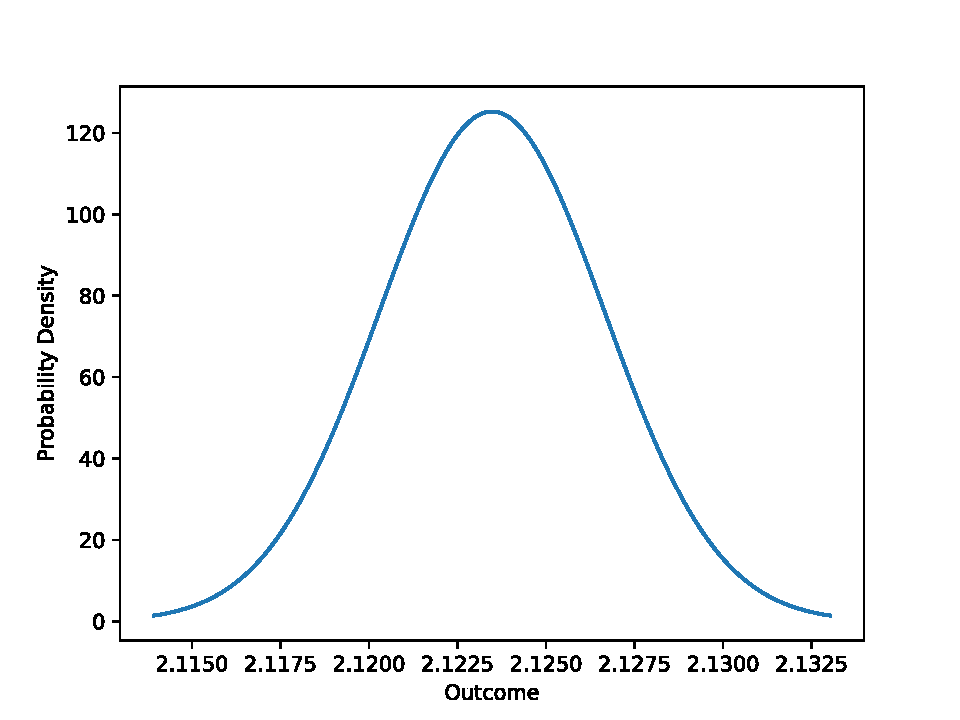
\includegraphics[width=0.8\linewidth]{./figures/Ch4_RidgeProbs}
    \caption{Gaussian RFQ count prediction prediction for a single output $y$}\label{Ch4Fig:RidgeProbs}
\end{figure}

Figure~\ref{Ch4Fig:RidgeProbs} plots the Gaussian prediction distribution of output $y$. The plot was produced based on a sample RFQ test data using a trained Bayesian Ridge model. This plot demonstrates the Bayesian nature of this model, with the peak being the most likely prediction of the count outcome.

    The prior for the coefficient $w$ is given by a zero mean Gaussian:
    \begin{equation}
        p(w|\lambda) = \mathcal{N} (w|0,\lambda^{-1}\mathbf{I}_p)
    \end{equation}
    $\alpha$ and $\lambda$ are both prior gamma distributions, with two versions for each as hyperparameters choice for Bayesian Ridge ($\alpha_1$, $\alpha_2$, $\lambda_1$ and $\lambda_2$).

    The L2 regularisation in Ridge regression is equivalent to a MAP (maximum posteriori) estimate using a Gaussian prior over the coefficients $w$ with precision $\lambda^{-1}$. $\lambda$ is known as the precision of the weights and it is possible to estimate it from the data. Similarly $\alpha$ which can also be estimated from the data and is referred to as the precision of the noise. This thesis used the scikit learn implementation \autocite{scikit-learn} of the supervised models above.
\end{description}

\subsection{Model implementation}

Figure~\ref{Ch4Fig:exp1_implement} highlights the main implementation steps followed for all three supervised learning models, each component is explained as follows:

\begin{enumerate}
    \item \text{Define hyperparameters} -- the first step involved defining the hyperparameter space. These are all the values which will be optimised using the cross-validation step. 
    \item \text{Cross-validation} -- this step returns the best hyperparameters by tuning the provided hyperparameters using a grid search technique. The chosen method was \texttt{GirdSearchCV} which iteratively considers all combinations of hyperparameters under a procedure called cross-validation. This experiment used a five-fold cross validation method where each model was trained on four of the folds used as training data and subsequently validated on the remaining one fold (Figure~\ref{Ch7Fig:1}). This process was repeated five times per model. The score and error measures reported from cross-validation were the average across all folds. 
    \item \text{Fit model} -- this step fits each of the candidate models using the chosen hyperparameters to the RFQ data matrix 'X' and the columnar matrix labels 'y'. This process quantifies the loss. This step now provides us with a trained model  i.e. the best model trained using the best hyperparameters.
    \item \text{Evaluate Best Model} -- the best model was evaluated on the entire training data once again as well as the test data and error and score measures were captured.
\end{enumerate}

\begin{figure}[!ht]\centering
    %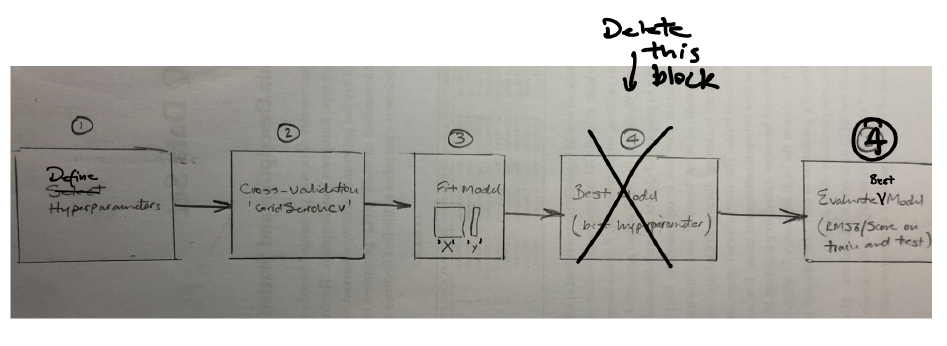
\includegraphics[width=1.0\linewidth]{./figures/sl_implementation}
    \resizebox{\linewidth}{!}{\begin{tikzpicture}[x=5cm,y=5cm]

        \begin{scope}[every node/.style={font=\footnotesize,rectangle,draw=black,fill=COL1,text width=3cm,minimum height=3cm,align=center}]
            \node (N1) at (1,0) {Define\\ hyperparameters};
            \node (N2) at (2,0) {Cross-validation `\texttt{GirdSearchCV}''};
            \node (N3) at (3,0) {Fit model\\\strut\\\strut\\\strut\\\strut\\};
            \node (N4) at (4,0) {Evaluate Best Model\\ (RMSE / Score on train and test)};
        \end{scope}

        \draw (2.8,-0.15) rectangle (3.0,0.05);
        \node[below,font=\footnotesize] at (2.9,-0.15) {`$x$'};
        \draw (3.1,-0.15) rectangle (3.2,0.05);
        \node[below,font=\footnotesize] at (3.15,-0.15) {`$y$'};

        \begin{scope}[-latex,line width=1pt]
            \draw (N1.east)--(N2.west);
            \draw (N2.east)--(N3.west);
            \draw (N3.east)--(N4.west);
        \end{scope}
        \foreach \n in {1,...,4} {\node[circle,draw,anchor=south,outer sep=5pt,font=\footnotesize] at (N\n.north) {\strut\n};};
    \end{tikzpicture}}
    \caption{Experiment 1 model implementation and evaluation methodology}\label{Ch4Fig:exp1_implement}
\end{figure}

During the implementation (Figure~\ref{Ch4Fig:exp1_implement}) phase this study examined the Ridge model to ascertain if it behaved as expected. The target variable Alpha (the regularisation strength) was varied and its effect on the calculated weights was plotted (Figure~\ref{Ch4Fig:weights_ridge}). The plot was based on a four hour count history. This exercise also helped with selecting Alphas in a range which reduced the variation in weights. As alpha tends to zero Ridge behaves like ordinary least squares (OLS) and is very noisy. As alpha increases the weight coefficients tend to zero as the shrinkage term effect dominates the loss expression. 

\begin{figure}[!ht]\centering
    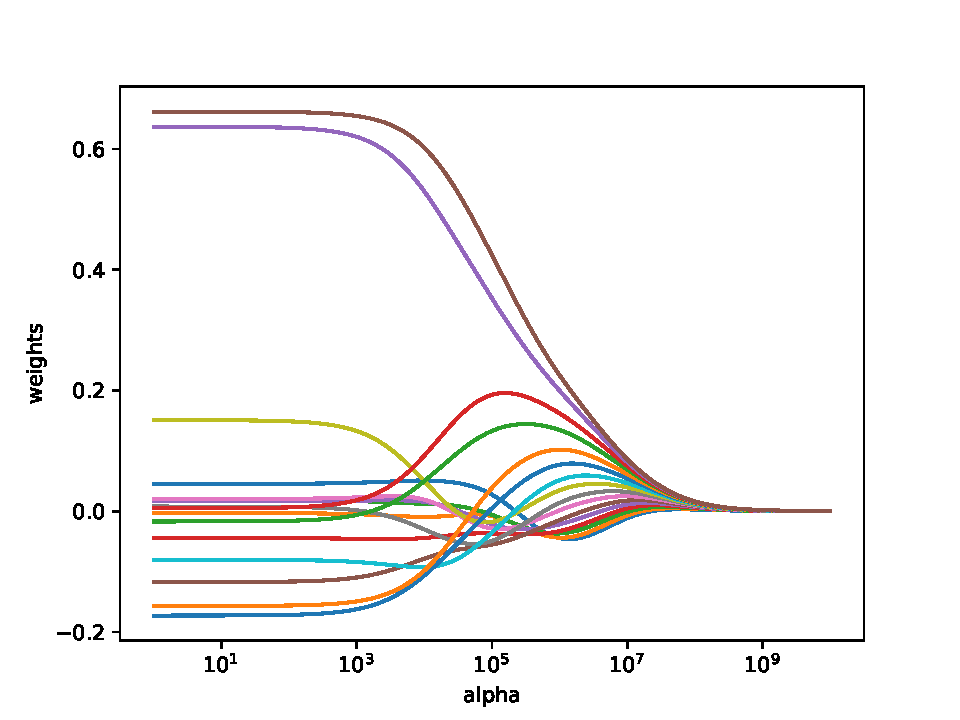
\includegraphics[width=0.8\linewidth]{./figures/ch4weights_ridge}
    \caption{Plot of ridge weights as a function of alpha, demonstrates Ridge behaves as expected}\label{Ch4Fig:weights_ridge}
\end{figure}




\subsection{Results and discussion}

The results of experiment 1 are shown in Table~\ref{Ch4Tab:1}. This table is based on the RFQ count histories of 30 minutes, 1 hour, 2 hours and 4 hours. The equivalent results for count and notional is presented in \textcolor{red}{Appendix [xx]}. 
The evaluation metrics of choice were RMS (root mean square) error (Expression~\ref{RMSE}) and $R^2$ Score. These two measures were reported for all three models on the train and test sets for all RFQ count and RFQ `count and history' data files. RMS error presents the standard deviation of the model prediction errors. It was chosen as a measure because it gives greater weighting to larger errors versus for example a mean average error (MAE) measure. $R^2$ Score (also called coefficient of determination) is often used for regression models. The best models have a score of 1.0, constant models despite variations in features would be scored as 0. Note $R^2$ can also be negative if the model is arbitrarily worse.

\begin{equation}\label{RMSE}
    \text{RMS Error} = \sqrt{\dfrac{1}{n} \sum_{i=1}^{n} {\left( {y}^{(i)} - {\hat{y}}^{(i)} \right)}^{2}}
\end{equation}


\begin{table}[!ht]\centering\small
    \caption{Experiment 1 -- Results table for RFQ counts}\label{Ch4Tab:1}
    \begin{tabular}{llccccc}
        \toprule
              &         & RMS   & RMS   & $R^2$ & $R^2$  \\
              & History & Error & Error & Score      & Score       \\
        Model & Length  & Train & Test  & Train      & Test        \\
        \midrule
        MLP Regressor
              & 30 mins & 4.14  & 4.17  & 0.98       & 0.97        \\
              & 1 hour  & 3.05  & 3.17  & 0.99       & 0.98        \\
              & 2 hours & 2.28  & 2.64  & 0.99       & 0.99        \\
              & 4 hours & 2.27  & 2.51  & 0.99       & 0.99        \\
        \midrule
        Ridge Regression
              & 30 mins & 4.22  & 4.23   & 0.97     &  0.97           \\
              & 1 hour  & 3.42  & 3.49   & 0.98    &  0.98          \\
              & 2 hours & 3.22  & 3.30    & 0.98    &  0.98           \\
              & 4 hours & 3.20   & 3.29   & 0.99    &   0.98          \\
        \midrule
        Bayesian Ridge Regression
              & 30 mins & 4.22  & 4.23   & 0.97     &  0.97           \\
              & 1 hour  & 3.42  & 3.49   & 0.98     &   0.98           \\
              & 2 hours & 3.22  & 3.30    & 0.98      &    0.98          \\
              & 4 hours & 3.20   &3.29    & 0.99     &    0.98          \\      
        \bottomrule
    \end{tabular}
\end{table}

Table~\ref{Ch4Fig:2} presents the best hyperparameters found after performing cross-validation on the count data. They are the parameters which were used when evaluating all three models to obtain the RMS error and $R^2$ Scores in Table~\ref{Ch4Tab:1}. The equivalent of Table~\ref{Ch4Fig:2} for both count and notional features is presented in \textcolor{red}{Appendix [xx]}

\begin{table}[!ht]\centering\footnotesize
    \caption{Experiment 1 -- hyperparameters chosen for model evaluation of the historical RFQ count data}\label{Ch4Fig:2}
    %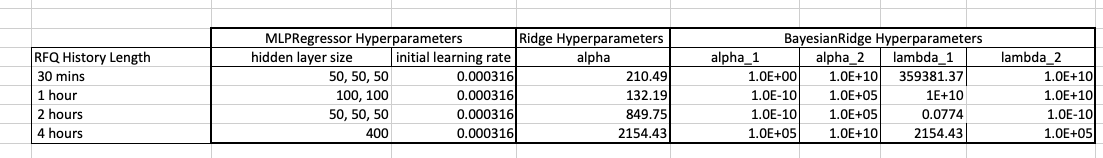
\includegraphics[width=1.2\linewidth]{./figures/Ch4_best_hyperprms_c}
    \resizebox{\linewidth}{!}{\begin{tabular}{lcccccccccc}
        \toprule
        &&
        \multicolumn{2}{c}{MLP Regressor} &&
        \multicolumn{1}{c}{Ridge} &&
        \multicolumn{4}{c}{Bayesian Ridge} \\
        &&
        \multicolumn{2}{c}{Hyperparameters} &&
        \multicolumn{1}{c}{Hyperparameters} &&
        \multicolumn{4}{c}{Hyperparameters} \\
        \cmidrule{3-4}\cmidrule{6-6}\cmidrule{8-11}
        RFQ     && hidden     & initial  &&         &&             &            &            &             \\
        History && layer      & learning &&         &&             &            &            &             \\
        Length  && size       & rate     && alpha   && alpha$_1$   & alpha$_2$  & lambda$_1$ & lambda$_2$  \\
        \midrule
        30 mins && 50, 50, 50 & 0.000316 && 210.49  && \num{1e0}   & \num{1e10} & 359381.37  & \num{1e10}  \\
        1 hour  && 100, 100   & 0.000316 && 132.19  && \num{1e-10} & \num{1e5}  & \num{1e10} & \num{1e10}  \\
        2 hours && 50, 50, 50 & 0.000316 && 849.75  && \num{1e-10} & \num{1e5}  & 0.0774     & \num{1e-10} \\
        4 hours && 400        & 0.000316 && 2154.43 && \num{1e5}   & \num{1e10} & 2154.43    & \num{1e5}   \\
        \bottomrule
    \end{tabular}}
\end{table}


\begin{figure}[!ht]\centering
    %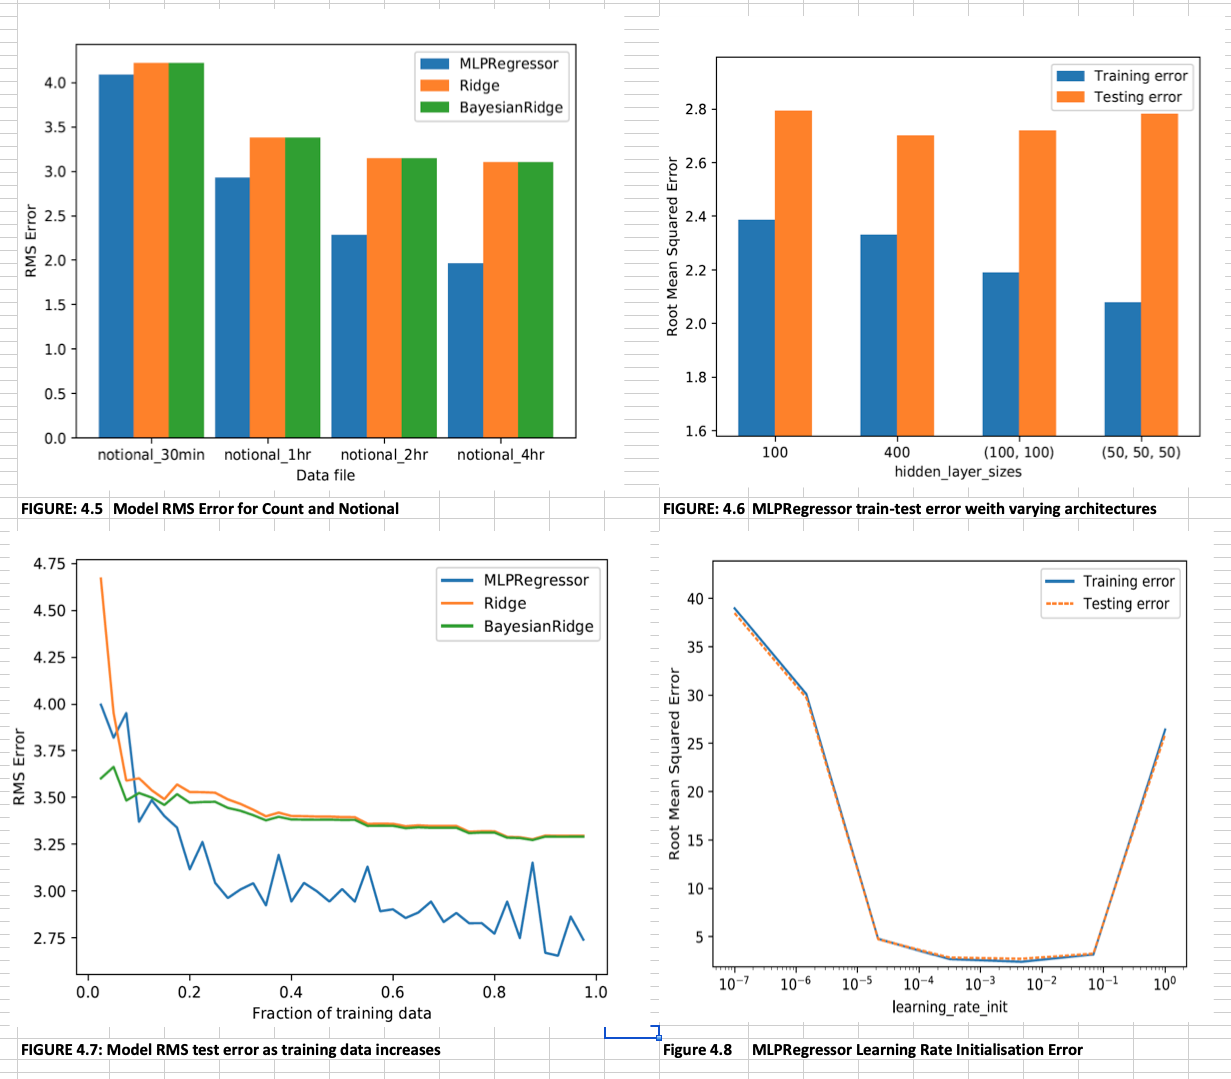
\includegraphics[width=1.0\linewidth]{./figures/exp1_combi_plots}
    \begin{subfigure}[t]{.475\linewidth}\centering
        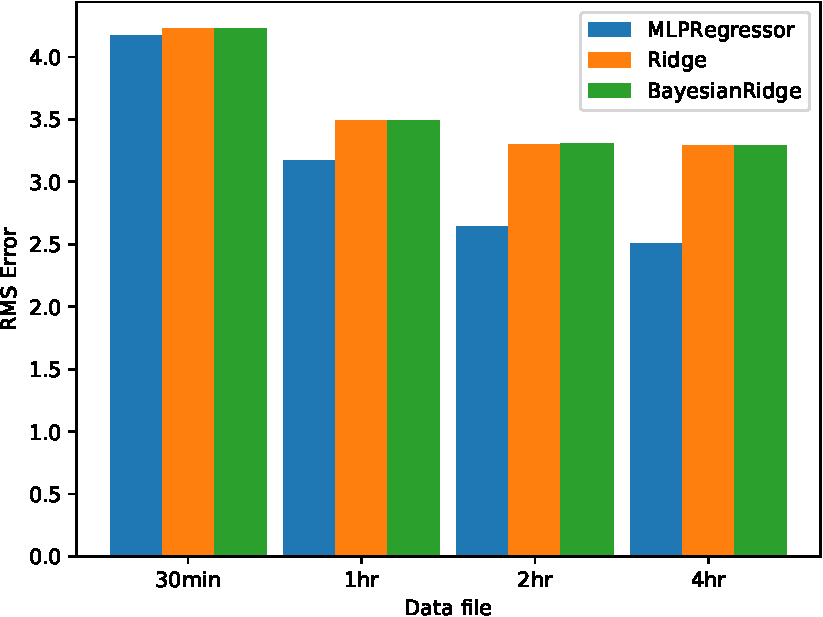
\includegraphics[width=1\linewidth]{./figures/Ch4fig5a}
        \caption{Model RMS test errors for count}\label{Ch4Fig:3a}
    \end{subfigure}\hfill%
    \begin{subfigure}[t]{.475\linewidth}\centering
        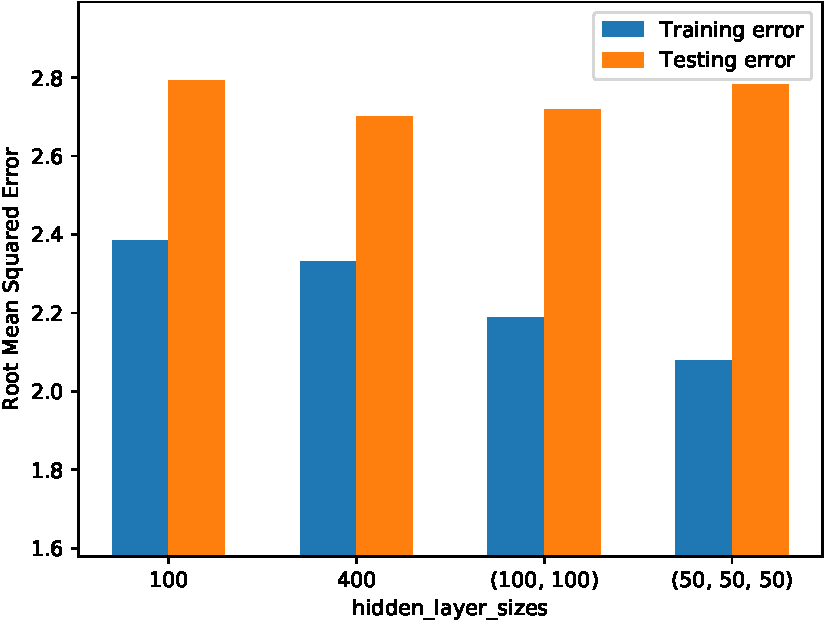
\includegraphics[width=1\linewidth]{./figures/Ch4fig5b}
        \caption{MLPRegressor RMS error vs. hidden layers using 4 hour count history}\label{Ch4Fig:3b}
    \end{subfigure}\\
    \strut\\
    \begin{subfigure}[t]{.475\linewidth}\centering
        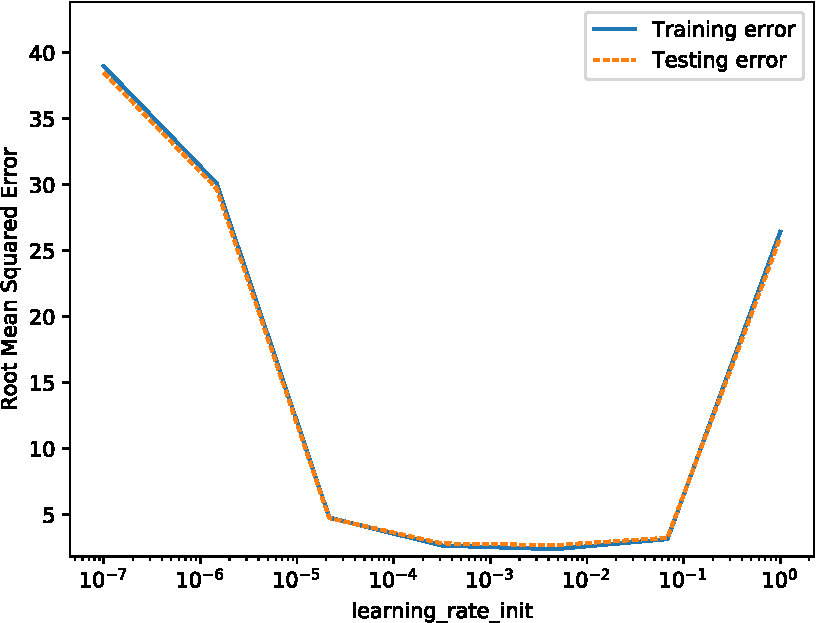
\includegraphics[width=1\linewidth]{./figures/Ch4fig5d}
        \caption{MLPRegressor RMS error vs. initial learning Rate hyperparameter using 4 hour count}\label{Ch4Fig:3c}
    \end{subfigure}\hfill%
    \begin{subfigure}[t]{.475\linewidth}\centering
        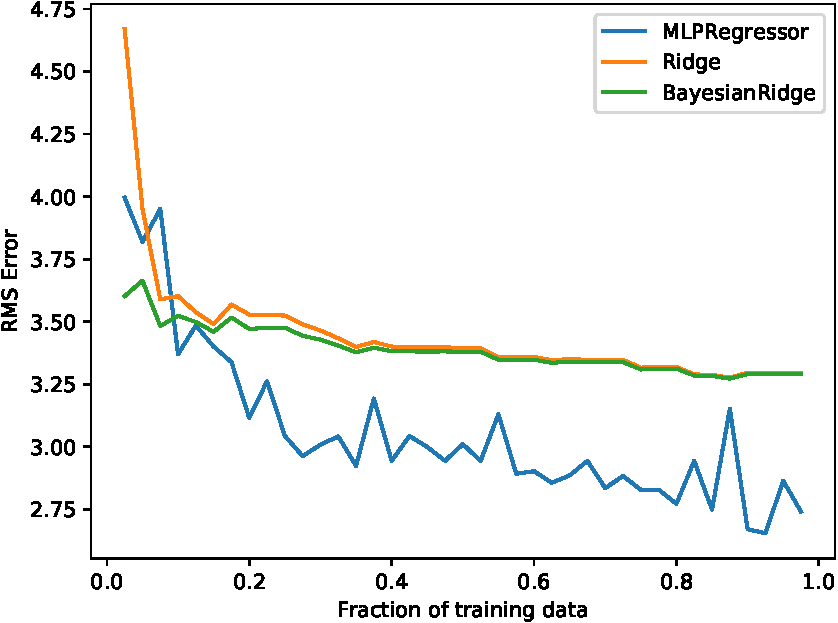
\includegraphics[width=1\linewidth]{./figures/Ch4fig5c}
        \caption{Model RMS test error vs. training data size for 4 hour count and notional}\label{Ch4Fig:3d}
    \end{subfigure}%
    \caption{Experiment 1 -- selected results plots}\label{Ch4Fig:3}
\end{figure}

Table~\ref{Ch4Fig:2} demonstrates that MLPRegressor (the neural network) model outperforms both Ridge and Bayesian Ridge particularly for larger histories. This is not surprising as neural networks are more powerful models for predictions versus linear models. The coefficient of determination score $R^2$ score has is very high i.e close to 1 for all models and files. This indicates that all models fit the all data files very well. The discussion of results in Table~\ref{Ch4Fig:2} will focus mainly on RMS errors as there is very little variance in $R^2$. 

The RMS error score for MLPRegressor indicates a lower standard deviation of the model prediction errors across all histories, versus Ridge and Bayesian Ridge. Both Ridge and Bayesian Ridge perform very similarly in terms of errors. Figure~\ref{Ch4Fig:3a} plots test RMS error for all three models across four count histories. MLPRegressor performs better overall and particularly when there are longer histories. Whereas Ridge and Bayesian Ridge only improve in error by a smaller fraction as the history increase from 30 minutes to 4 hours.

Analysing MLPRegressor further, Figure~\ref{Ch4Fig:3b} shows the impact of different hidden layer architectures in the network on the RMS error. This plot was based on a 4 hour count history where `100' represents a single hidden layer formed of 100 neurons and `50, 50, 50' represents 3 hidden layers of length 50 neurons each. The plot shows that the more layers in the network the better the fit on the train data, however a single hidden layer with `400' neurons has the lowest test error.

Figure~\ref{Ch4Fig:3c} plots the performance of of a range of initial learning rate values versus RMS error for both the train and test sets. This was based on a 4 hour RFQ count history. The initial learning rate controls the step size during gradient descent for both `sgd' and `Adam' solvers (Experiment 1 used `Adam'). It shows that an initial learning which is set too high ($>10^{-1}$) or too low ($<10^{-5}$) is not optimal for learning and results in a poor prediction and hence a large error. The optimal set of learning rates for initialisation are between $10^{-3}$ and $10^{-2}$. The plot also shows that the train and test errors are very similar suggesting that MLPRegressor generalises well to the test data. Similar analysis was performed on hyperparameters for Ridge (alpha) and Bayesian Ridge (alpha$_1$, alpha$_2$, lambda$_1$, lambda$_2$). For Ridge, it was found that train and test RMS error were almost identical for values of alpha from  $10^{-11}$ to $10^{4}$, and beyond $10^{4}$ the RMS error increased from below 5 to around 25 (Figure~\ref{App:A4a}. For Bayesian Ridge lambda$_1$ showed a similar step change behaviour to Ridge in RMS error. For lambda$_1$ values from  $10^{-10}$ to  $10^{1}$ the RMS error was less than 5, above $10^{1}$ the RMS error increased to over 25 (Figure~\ref{App:A4b}.

Figure~\ref{Ch4Fig:3d} compares the RMS test error for all 3 models versus the size of the training data. Overall we observe consistent behaviour where MLPRgressor outperforms Ridge and Bayesian Ridge and all three models perform better in the presence of more training data which is perhaps expected. Interestingly Ridge perform better than Bayesian Ridge in the presence of less training data but they converge to the same error as we use $100\%$ of the training data. 


Table~\ref{Ch4Fig:2} displays the hyperparameters provided to each model (the hyperparameters not given would assume default values). For each length of count history it presents the best hyperparameter value selected for each model using the cross-validation \texttt{GridSearchCV} method. These hyperparmaeters were then use in the `best model' which was evaluated on the training and test data sets to report the RMS error and $R^2$ scores in Table~\ref{Ch4Tab:1}.



\subsection{Conclusion}

Experiment 1 demonstrates that all three supervised models are able to predict RFQ counts to a high degree and they generalise well to the test set. MLPRegressor is clearly a better predictor of RFQ data compared to Ridge and Bayesian Ridge, with an RMS error of only $2.27$ for a 4 hour history.  MLPRegressor RMS error has greater sensitivity to the hyperparameters chosen, namely the initial learning rate and the hidden layers. Whereas Ridge and Bayesian Ridge were found to be fairly insensitive to hyperparatmeters except for very large values of alpha and lambda$_1$. It is also evident that the presence more training data greatly reduces the RMS test errors observed.


\section{Experiment 2 - predicting RFQs using the Bayesian unsupervised hidden Markov model}

\subsection{Introduction}

Although Experiment 2 is about predicting RFQs, it should be noted that the hidden Markov model (HMM) is able to give much more sophisticated insight into the underlying process, as Experiment 3 will demonstrate. In theory, for prediction, a first order Markov chain (Figure~\ref{Ch2Fig:5}) could be used, however what the HMM model gives beyond a simple Markov chain is the ability to infer and reason about hidden states. An example of a HMM model set-up for predicting RFQs is provided in Figure~\ref{Ch7Fig:9}, where visible RFQ $v_3$ can be predicted having just observed visible RFQs $v_0\text{:}v_2$. 

%\begin{figure}[!ht]\centering
%    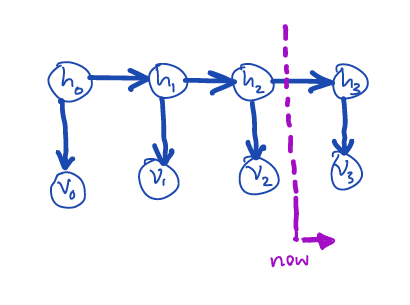
\includegraphics[width=0.5\linewidth]{./figures/Ch7fig1}
%    \caption{Example hidden Markov model where the 4th visible variable is predicted}\label{Ch7Fig:3}
%\end{figure}

\begin{figure}[!ht]\centering
    %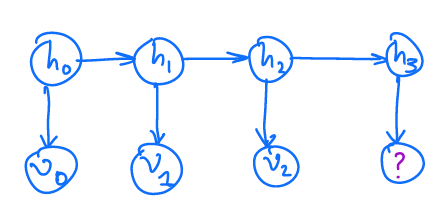
\includegraphics[width=0.5\linewidth]{./figures/Ch7fig7}
    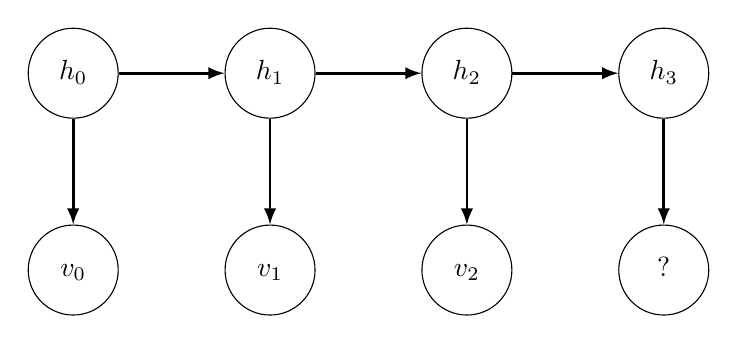
\begin{tikzpicture}[x=2.5cm,y=2.5cm]
        \begin{scope}[every node/.style={circle,draw,text width=20pt,align=center}]
            \node (h0)  at (0.0,1) {\strut$h_0$};
            \node (h1)  at (1.0,1) {\strut$h_1$};
            \node (h2)  at (2.0,1) {\strut$h_2$};
            \node (h3)  at (3.0,1) {\strut$h_3$};

            \node (v0)  at (0.0,0) {\strut$v_0$};
            \node (v1)  at (1.0,0) {\strut$v_1$};
            \node (v2)  at (2.0,0) {\strut$v_2$};
            \node (v3)  at (3.0,0) {\strut?};
        \end{scope}
        \begin{scope}[line width=1pt,-latex]
            \draw (h0.east)--(h1.west);
            \draw (h1.east)--(h2.west);
            \draw (h2.east)--(h3.west);
            \foreach \n in {0,1,2,3} {\draw (h\n.south)--(v\n.north);}
        \end{scope}
    \end{tikzpicture}
    \caption{Hidden Markov model set-up to predict RFQ visible variable `$v_3$'}\label{Ch7Fig:9}
\end{figure}



\subsection{Model implementation}

In this application it turns out the HMM is not the best tool for predicting the next RFQ. Theoretically it is possible to make predictions via the hidden states of the HMM. Using Figure~\ref{Ch7Fig:9} as an example framework, it is possible predict what the RFQ count is at $v_3$ having just observed visible RFQs $v_0\text{:}v_2$. This achieved by calculating the conditional probability $p(v_3| v_0,v_1,v_2)$

The HMM in Figure~\ref{Ch7Fig:9} can be written as the expression below to make use of message passing inference:

\begin{multline}
    p(h_0,h_1,h_2,h_3,v_0,v_1,v_2,v_3) =\\
    p (h_0)     \!\!\cdot\!\!
    p (v_0|h_0) \!\!\cdot\!\!
    p (h_1|h_0) \!\!\cdot\!\!
    p (h_2|h_1) \!\!\cdot\!\!
    p (h_3|h_2) \!\!\cdot\!\!
    p (v_1|h_1) \!\!\cdot\!\!
    p (v_2|h_2) \!\!\cdot\!\!
    p (v_3|h_2)
\end{multline}

Where the proportionality below holds once the normalisation constant has been removed:
\begin{equation}
    p(v_3|v_0,v_1,v_2) \propto \sum_{h_0,h_1,h_2,h_3} p (h_0,h_1,h_2,h_3,v_0,v_1,v_2,v_3)
\end{equation}

It should be noted that the HMM being a Bayesian could easily cope with missing data (unlike the classical methods). This property was used in the implementation where it was shown that it is possible to substitute any number with a \texttt{nan} and the model copes. It handles missing data by summing out probabilities, for example in the presence of three data points and where one was missing it could simply sum out the missing variable. For instance in the expression below variable `a' could be summed out if it was missing.

\begin{equation}
    \sum_{a} p (a,b,c) = p (b,c)
\end{equation}

\begin{figure}[!ht]\centering
    %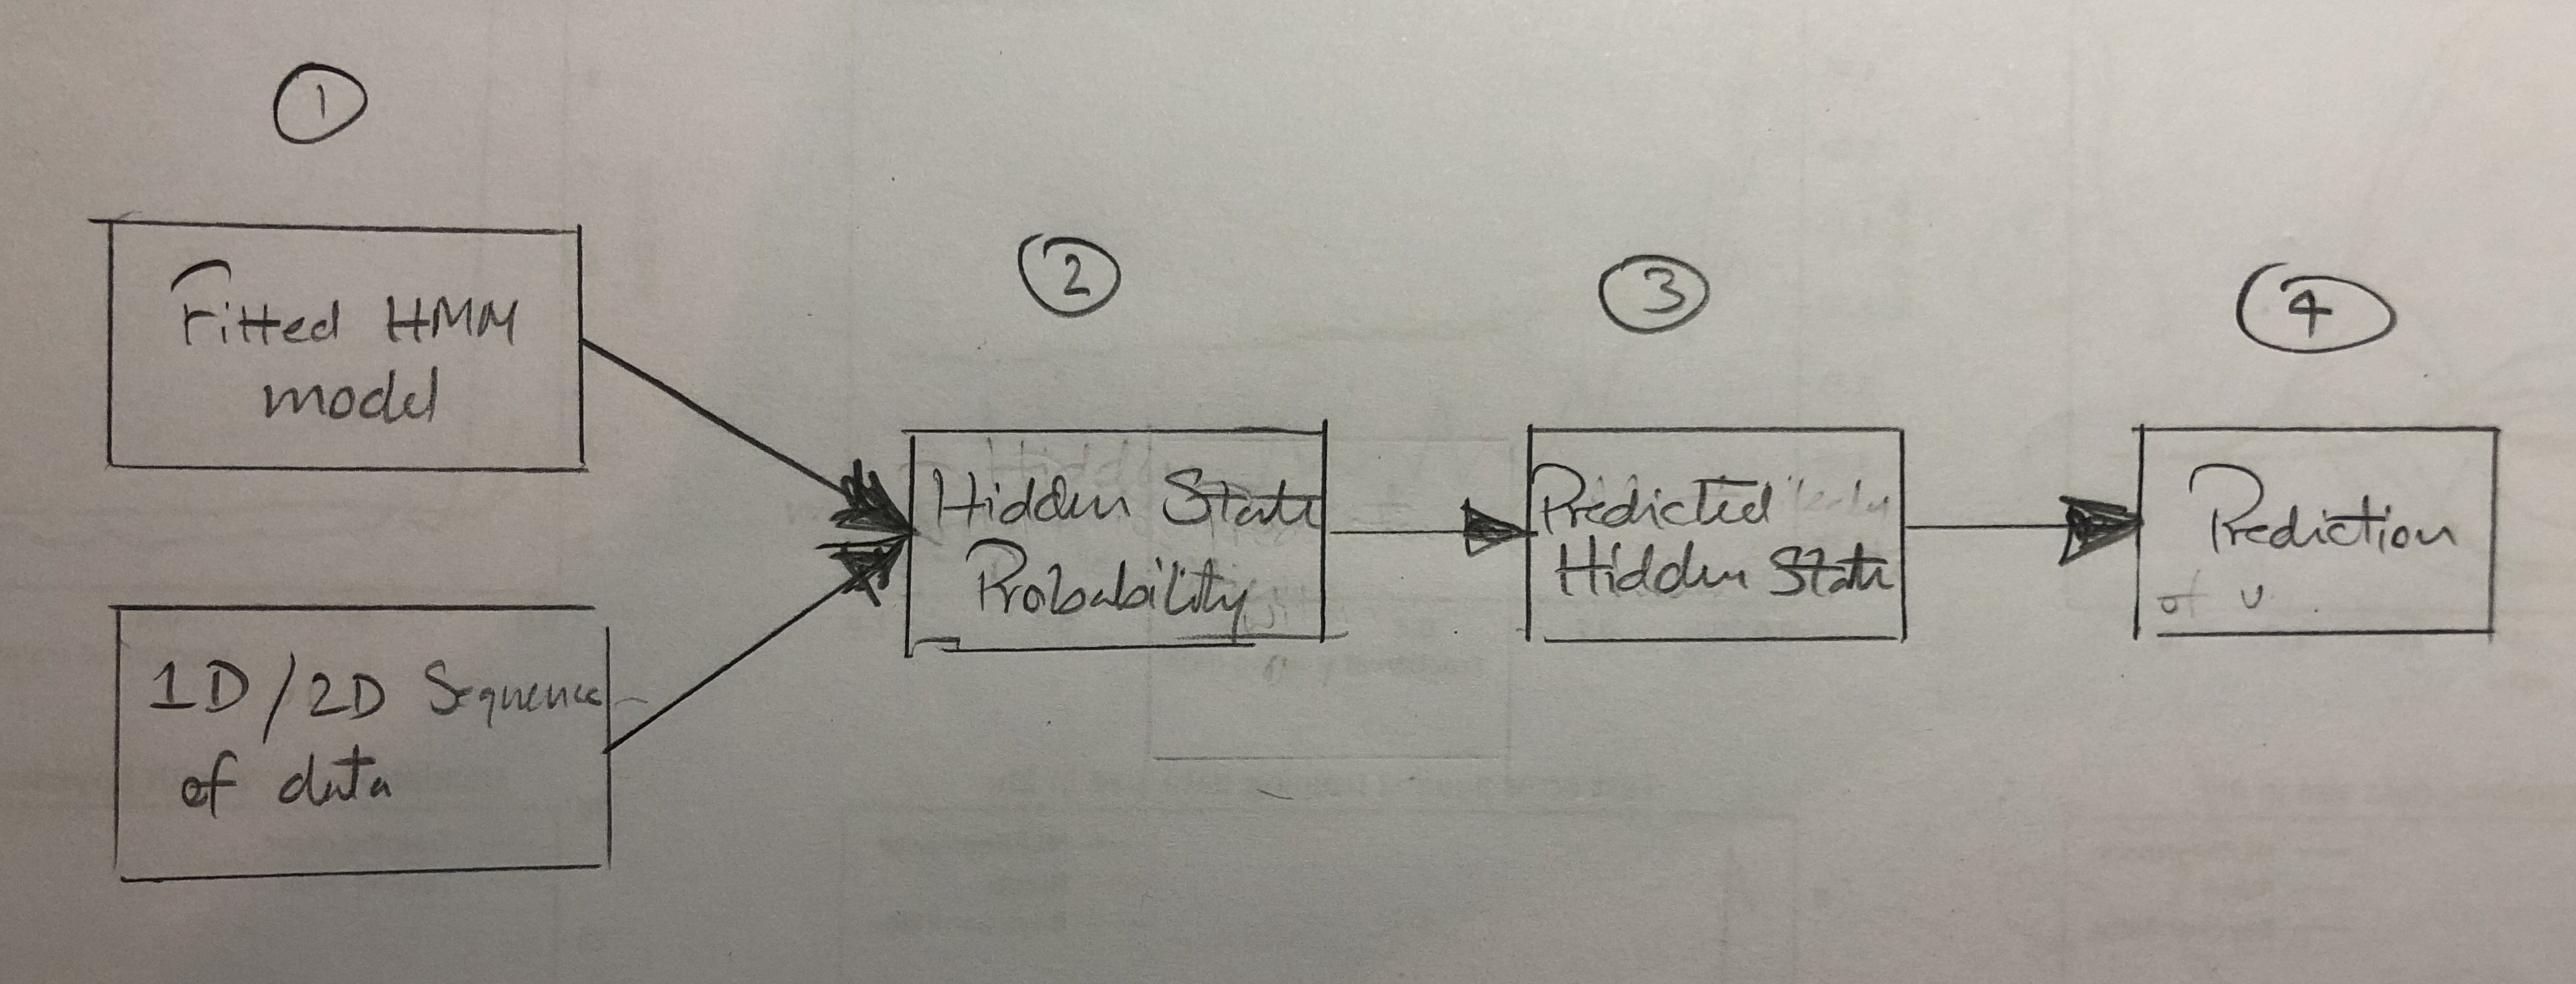
\includegraphics[width=1.0\linewidth]{./figures/predict_hmm}
    \resizebox{\linewidth}{!}{\begin{tikzpicture}[x=5cm,y=5cm]
        \begin{scope}[every node/.style={font=\footnotesize,rectangle,draw=black,fill=COL1,text width=3cm,minimum height=2cm,align=center}]
            \node (N1) at (1,0.3)  {Fitted\\ HMM Model};
            \node (N1b) at (1,-0.3) {1D/2D\\ Sequence of data};
            \node (N2) at (2,0) {Hidden State\\ Probability};
            \node (N3) at (3,0) {Predicted\\ Hidden State};
            \node (N4) at (4,0) {Prediction};
        \end{scope}

        \begin{scope}[-latex,line width=1pt]
            \draw (N1.east)--(N2.170);
            \draw (N1b.east)--(N2.190);
            \draw (N2.east)--(N3.west);
            \draw (N3.east)--(N4.west);
        \end{scope}
        \foreach \n in {1,...,4} {\node[circle,draw,anchor=south,outer sep=5pt,font=\footnotesize] at (N\n.north) {\strut\n};};
    \end{tikzpicture}}
    \caption{Implementation steps to predicting next RFQ using the HMM model}\label{Ch4Fig:predict_hmm}
\end{figure}

Following on from the theory, below describes the implementation steps in Figure~\ref{Ch4Fig:predict_hmm} which use the HMM model to predict RFQs:

\begin{enumerate}
    \item \text{Fit HMM model on 1 and 2 dimensional sequences} -- to begin with it is necessary to create and fit a HMM model. The HMM model is then able to consume both 1-dimensional RFQ count sequence (1D per Figure~\ref{Ch4Fig:6}) and 2-dimensional RFQ count and notional sequence (2D per Figure~\ref{Ch4Fig:67}). 
    
    \item \text{Hidden state probability} -- the probability of each hidden state at the end of the sequence of data is obtained.
    
    \item \text{Predicted hidden state} -- this step calculates the probability of the hidden states at the next time step using a defined transition matrix.
    
     \item \text{Prediction} -- finally a RFQ prediction is made by selecting the most likely state by using the mean of its emission distribution.
\end{enumerate}    

\subsection{Results and Discussion}

Table~\ref{Ch4Fig:hmm_predict_error} presents the RMS errors for prediction of RFQs based on `differences' sequences taken from the data split of train and test. The sequences used were 2,4,6 and 8 in length equivalent to 30 minutes, 1 hour, 2 hours and 4 hours. This was performed for both `count' sequences and `count and notional' RFQ sequences. 

The test errors marginally improve when using 2D data (i.e. when also incorporating notional sequences) when predicting using shorter sequences, however surprisingly as the history lengthens, only the `count' sequences improve in error compared to 'count and notional' where the error get marginally worse using longer sequences. In comparison to Experiment 1, the HMM model performs worse than all three supervised models with an average RMS error of 4.40 for count.


\begin{table}[!ht]\centering\small
    \caption{Hidden Markov model RFQ prediction error}\label{Ch4Fig:hmm_predict_error}
    %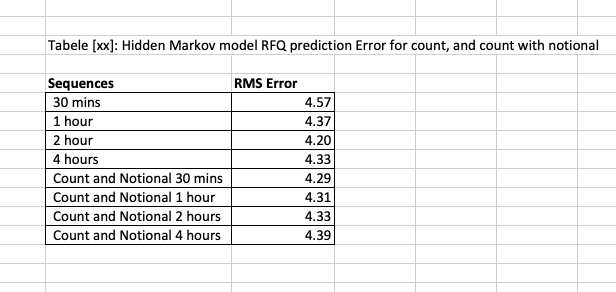
\includegraphics[width=1.0\linewidth]{./figures/Exp2_resultstable}
    \begin{tabular}{lcc}
        \toprule
            Sequences  & RMS Train Error & RMS Test Error \\
        \midrule
            30 mins                    & 4.59 & 4.57 \\
            1 hour                     & 4.40 & 4.37 \\
            2 hours                    & 4.21 & 4.20 \\
            4 hours                    & 4.19 & 4.33 \\
            Count and Notional 30 mins & 4.26 & 4.29 \\
            Count and Notional 1 hour  & 4.26 & 4.31 \\
            Count and Notional 2 hours & 4.26 & 4.33 \\
            Count and Notional 4 hours & 4.27 & 4.39 \\
        \bottomrule
    \end{tabular}
\end{table}

\subsection{Conclusion}

Experiment 2 demonstrated that it is possible to make use of the hidden Markov model to make RFQ predictions by using sequences of `differences'. Although the hidden Markov model does not appear to predict as well the supervised models due to larger RMS errors. Hence, Experiment 3 attempts to make more insightful use of the the HMM model and its hidden states to reason about the underlying RFQ market regime.

\section{Experiment 3 - Inferring RFQ hidden states using the hidden Markov model}

\subsection{Introduction}

There are two possible approaches for the set-up in Experiment 3. Firstly using our domain knowledge to subjectively impose an emission and transition matrix and instead of training those using the processes of `filtering' and the `Viterbi' algorithm to infer the most likely path. The second option is to use the EM algorithm to train our model, where the EM algorithm would perturb the emission and transitions distributions as well as the `prior' to find the set which best fits the data. This thesis uses the EM learning approach.

\subsection{Model implementation}

\begin{figure}[!ht]\centering
    %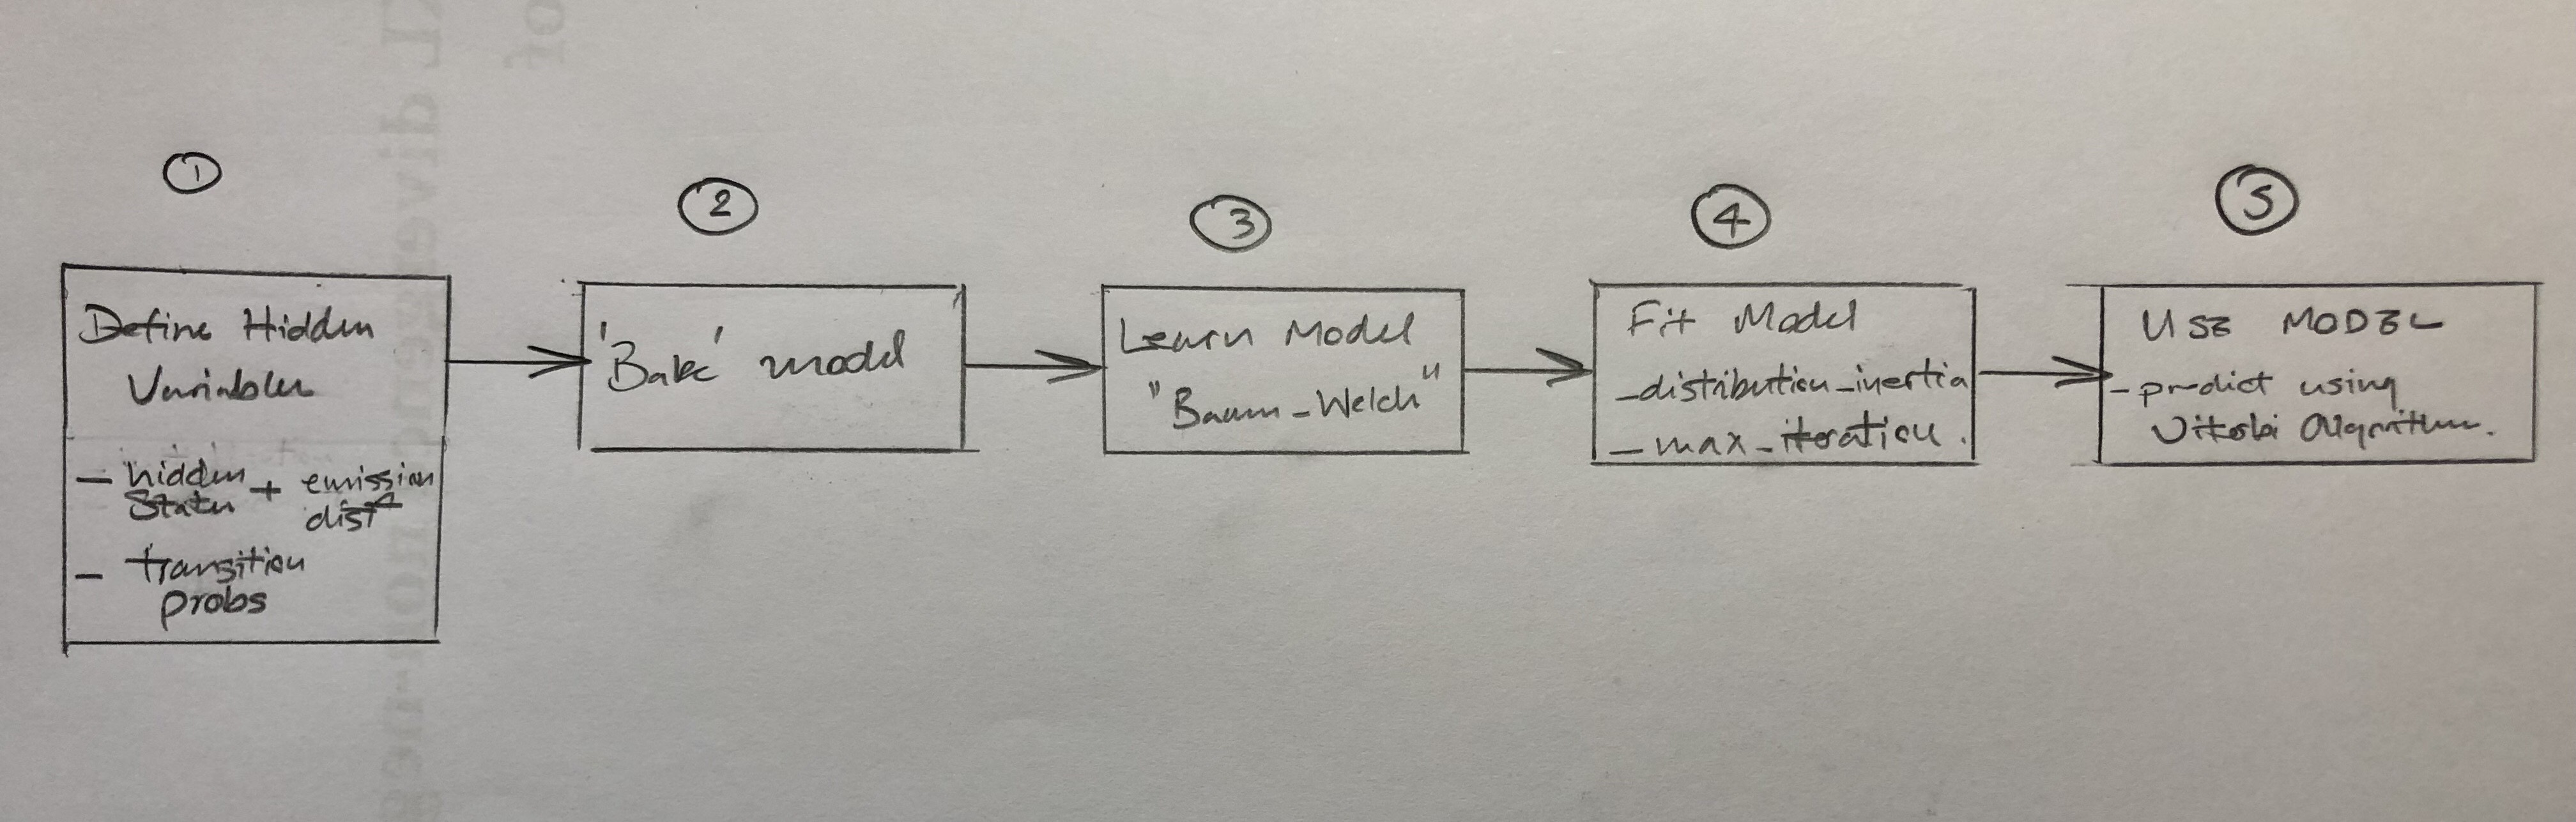
\includegraphics[width=1.0\linewidth]{./figures/hmm_inference}
        \resizebox{\linewidth}{!}{\begin{tikzpicture}[x=4.7cm,y=5cm]
        \begin{scope}[every node/.style={font=\footnotesize,rectangle,draw=black,fill=COL1,text width=3.3cm,minimum height=3.3cm,align=center}]
            \node (N1) at (1,0) {Define\\ Hidden Variables
            \begin{itemize}[leftmargin=*,noitemsep]
                \item hidden state + emission distribution
                \item transition probabilities
            \end{itemize}};
            \node (N2) at (2,0) {`Bake' model};
            \node (N3) at (3,0) {Learn Model\\ ``Baum-Welch''};
            \node (N4) at (4,0) {Fit Model};
            % \begin{itemize}[leftmargin=*,noitemsep]
            %     \item distribution
            %     \item inertia
            %     \item max\_iteration
            % \end{itemize}};
            \node (N5) at (5,0) {Use Model
            \begin{itemize}[leftmargin=*]
                \item predict\\ using Viterbi\\ algorithm
            \end{itemize}};
        \end{scope}

        \begin{scope}[-latex,line width=1pt]
            \draw (N1.east)--(N2.west);
            \draw (N2.east)--(N3.west);
            \draw (N3.east)--(N4.west);
            \draw (N4.east)--(N5.west);
        \end{scope}
        \foreach \n in {1,...,5} {\node[circle,draw,anchor=south,outer sep=5pt,font=\footnotesize] at (N\n.north) {\strut\n};};
    \end{tikzpicture}}
    \caption{HMM model inference implementation steps for 1D and 2D sequences}\label{Ch4Fig:1}
\end{figure}


Experiment 3 involved two different implementations for inference, based on 1-dimensional count `difference' sequences and 2-dimensional `count and notional' difference sequences. Figure~\ref{Ch4Fig:6} shows the set up for a HMM model with three hidden states and three corresponding visible states (1D). The 2-dimensional (2D) implementation can be represented by the example in Figure~\ref{Ch4Fig:67} which is a HMM belief network with three hidden states, three visible states for `count' and likewise three for `notional'. The main implementation steps for both 1D and 2D are depicted in Figure~\ref{Ch4Fig:1}, a brief description is provided below, after which more detailed analysis follows:

\begin{enumerate}
    \item \text{Define Hidden Variables} -- to begin with prior to training the HMM model, it was necessary to define the initial values for the hidden regimes as well transition and emission matrices.
    
    \item \text{`Bake' model} -- this another term for creating the HMM model using the initialised values.
    
    \item \text{Learn Model} -- the Baum-Welch EM algorithm was used in this step, which forces the hidden states to assume the emission distributions of the underlying regime in the data (increasing, decreasing, level)
    \item \text{Fit Model} -- the HMM model is fitted on the training data sequence using the chosen hyperparameters (distribution inertia and maximum iteration)
    \item \text{Use Model} -- finally the `Viterbi' algorithm is used on the the model predictions to make inferences about the most likely hidden states i.e. the RFQ market regimes.
    
\end{enumerate}  


\begin{figure}[!ht]\centering
    \begin{subfigure}[t]{.475\linewidth}\centering
        %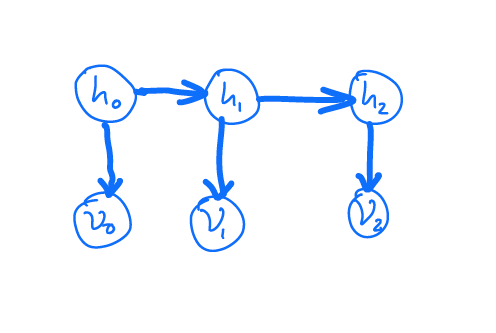
\includegraphics[width=0.8\linewidth]{./figures/Ch7fig4}
    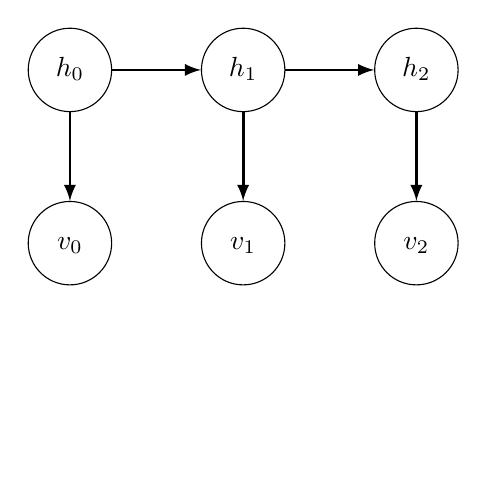
\begin{tikzpicture}[x=2.2cm,y=2.2cm]
        \begin{scope}[every node/.style={circle,draw,text width=17pt,align=center}]
            \node (h0)  at (0.0,1) {\strut$h_0$};
            \node (h1)  at (1.0,1) {\strut$h_1$};
            \node (h2)  at (2.0,1) {\strut$h_2$};

            \node (v0)  at (0.0,0) {\strut$v_0$};
            \node (v1)  at (1.0,0) {\strut$v_1$};
            \node (v2)  at (2.0,0) {\strut$v_2$};

            \node[opacity=0] (n0)  at (0.0,-1) {\strut};
            \node[opacity=0] (n1)  at (1.0,-1) {\strut};
            \node[opacity=0] (n2)  at (2.0,-1) {\strut};
        \end{scope}
        \begin{scope}[line width=1pt,-latex]
            \draw (h0.east)--(h1.west);
            \draw (h1.east)--(h2.west);
            \foreach \n in {0,1,2} {\draw (h\n.south)--(v\n.north);}
        \end{scope}
    \end{tikzpicture}

        \caption{Hidden Markov model with \mbox{1-dimensional} visible variables (count)}\label{Ch4Fig:6}
    \end{subfigure}\hfill%
    \begin{subfigure}[t]{.475\linewidth}\centering
        %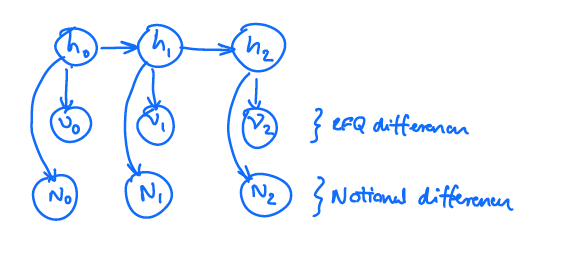
\includegraphics[width=0.8\linewidth]{./figures/Ch7fig5}
    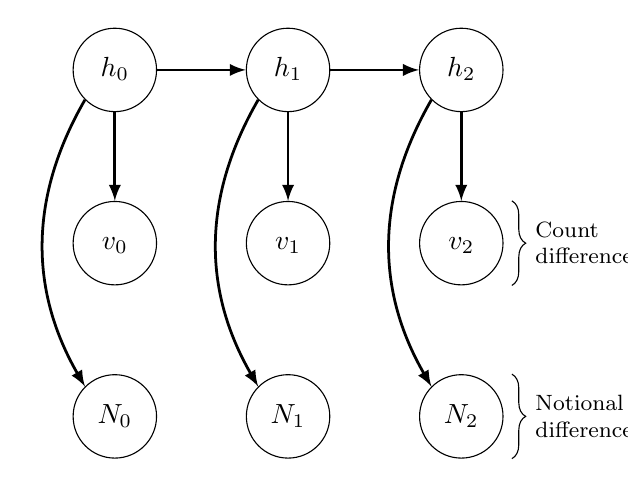
\begin{tikzpicture}[x=2.2cm,y=2.2cm]
        \begin{scope}[every node/.style={circle,draw,text width=17pt,align=center}]
            \node (h0)  at (0.0,1) {\strut$h_0$};
            \node (h1)  at (1.0,1) {\strut$h_1$};
            \node (h2)  at (2.0,1) {\strut$h_2$};

            \node (v0)  at (0.0,0) {\strut$v_0$};
            \node (v1)  at (1.0,0) {\strut$v_1$};
            \node (v2)  at (2.0,0) {\strut$v_2$};

            \node (n0)  at (0.0,-1) {\strut$N_0$};
            \node (n1)  at (1.0,-1) {\strut$N_1$};
            \node (n2)  at (2.0,-1) {\strut$N_2$};
        \end{scope}
        \begin{scope}[line width=1pt,-latex]
            \draw (h0.east)--(h1.west);
            \draw (h1.east)--(h2.west);
            \foreach \n in {0,1,2} {
                \draw (h\n.south)--(v\n.north);
                \draw (h\n.225) to[bend right] (n\n.135);
                }
        \end{scope}
        \draw [decorate,decoration={brace,amplitude=5pt}]
            ([shift={(3pt,0pt)}]v2.north-|v2.east) --
            ([shift={(3pt,0pt)}]v2.south-|v2.east)
            node [black,midway,right,xshift=5pt,text width=20pt,font=\footnotesize] {Count\\ differences};
        \draw [decorate,decoration={brace,amplitude=5pt}]
            ([shift={(3pt,0pt)}]n2.north-|n2.east) --
            ([shift={(3pt,0pt)}]n2.south-|n2.east)
            node [black,midway,right,xshift=5pt,text width=20pt,font=\footnotesize] {Notional\\ differences};
    \end{tikzpicture}
        \caption{Hidden Markov model with \mbox{2-dimensional} visible variables ('count and notional')}\label{Ch4Fig:67}
    \end{subfigure}
    \caption{}\label{Ch4Fig:678}
\end{figure}


Let us assume that our hidden states $h_n$ are all discrete variables, which reflect the three underlying regimes of RFQ market activity. In other words the underlying market regime will always be in any one of three states: `increasing', `decreasing' or `level' activity. This implies that the generation of RFQs, i.e. our `visible' count variable, is driven by the regime the market is currently in.

The transformation of RFQ data into a suitable state is absolutely critical for successful inferential modelling using the HMM. As mentioned previously unlike the supervised models there is no need to transform RFQs into labelled data sets of '$X$' and `$y$' for the HMM as it can deal with `un-labelled' sequences. However, we do need to ensure that the `visible' RFQ data is formulated in such a way which fits the HMM assumptions. The HMM model must obey the Markov assumption, i.e. the future depends on the present state and assumes that is a sufficient representation of history. That is another way of saying the present state is sufficient to decide what comes next. Therefore we are able to draw it as per the examples setup in Figure~\ref{Ch4Fig:6} which is a belief network embodiment of the Markov assumption where the relationship below holds:
\begin{equation}
    v_2 \bigCI v_1 | h_2
\end{equation}

Expression 4.10 means given `hidden' state $h_2$, our `visible' variable $v_2$ is independent of the past $v_1$. Armed with this knowledge the first attempt was to model the RFQs naively using the HMM model. Figure~\ref{Ch7Fig:4} below shows a series of RFQs over time with 3 labelled as $v_0$, $v_1$ and $v_2$, all three of which are in an increasing regime with corresponding hidden states for each.

\begin{figure}[!ht]\centering
    %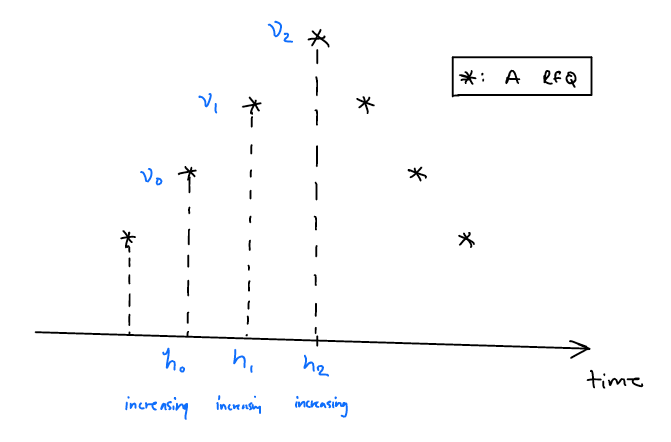
\includegraphics[width=0.5\linewidth]{./figures/Ch7fig2}
    \begin{tikzpicture}[x=40pt,y=40pt]
        \draw[->] (0,0)--(8,0) node[at end,below left] {time};
        \coordinate (O) at (0,0);
        \coordinate (n0) at (1,1);
        \coordinate (n1) at (2,2);
        \coordinate (n2) at (3,3);
        \coordinate (n3) at (4,4);
        \coordinate (n4) at (5,3);
        \coordinate (n5) at (6,2);
        \coordinate (n6) at (7,1);

        \coordinate (l) at (6.5,4);
        \node[right,inner sep=2pt,rectangle,draw,font=\footnotesize] at (l) {\textcolor{COL3}{\textbullet}~A RFQS};

        \foreach \n in {1,...,3} {\draw[dashed] (O-|n\n) -- (n\n);}
        \foreach \n in {0,...,6} {\fill[COL3] (n\n) circle (2pt);}
        \begin{scope}[every node/.style={above left,inner sep=2pt,font=\footnotesize}]
            \node at (n1) {$v_0$};
            \node at (n2) {$v_1$};
            \node at (n3) {$v_2$};
        \end{scope}
        \begin{scope}[every node/.style={below,inner sep=2pt,font=\footnotesize}]
            \node (h0) at (n1|-O) {$h_0$};
            \node (h1) at (n2|-O) {$h_1$};
            \node (h2) at (n3|-O) {$h_2$};
        \end{scope}
        \begin{scope}[every node/.style={below,inner sep=5pt,font=\scriptsize}]
                \node at (h0) {increasing};
                \node at (h1) {increasing};
                \node at (h2) {increasing};
        \end{scope}
    \end{tikzpicture}
    \caption{RFQs in an `increasing' regime}\label{Ch7Fig:4}
\end{figure}

\subsubsection{`Differences' methodology}

Next it is important to ascertain if our real world knowledge of the RFQ data is aligned with our knowledge of a HMM model. i.e. does the RFQ data obey the Markovian assumption of $v_2 \bigCI v_1 | h_2$ imposed by our HMM model?\\

Figure~\ref{Ch7Fig:4} clearly shows that the Markovian assumption does not hold and that $v_2$ is not independent from $v_1$ given $h_2$ i.e.: $v_2 \notbiCI v_1 | h_2$. The reason for that is that given $h_2$ is in an increasing regime, $v_2$ is highly likely to be greater than $v_1$. Therefore because knowing $v_1$ tells us something about $v_2$ this means they are not independent. Hence, we propose to take a ``differences'' approach. Transforming our RFQ data into a `differences' universe is much more likely to to make $v_2$ independent from $v_1$ given the regime we are in. Therefore, the ``differences'' approach is much more suitable for a HMM model as the Markov assumption holds.

\begin{figure}[!ht]\centering
    %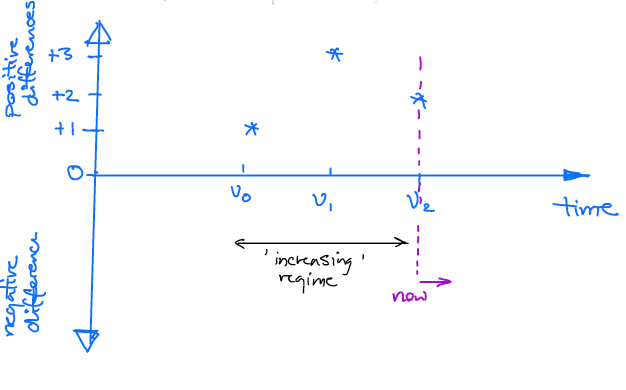
\includegraphics[width=0.5\linewidth]{./figures/Ch7fig3}
        \begin{tikzpicture}[x=40pt,y=40pt]
        \draw[->] (0,0)--(8,0) node[at end,below left] {time};
        \draw[->] (0,-2)--(0,4);

        \coordinate (O) at (0,0);
        \coordinate (Ob) at (0,-1.5);
        \coordinate (Ot) at (0,2.5);
        \coordinate (v0) at (2.5,1);
        \coordinate (v1) at (4,3);
        \coordinate (v2) at (5.5,2);

        \coordinate (l) at (5.5,3.5);
        \node[right,inner sep=2pt,rectangle,draw,font=\footnotesize] at (l) {\textcolor{COL3}{\textbullet}~RFQ differences};

        \foreach \n in {0,...,2} {
            \fill[COL3] (v\n) circle (2pt);
            \draw (O-|v\n)--++(270:5pt) node[at end,below,font=\footnotesize] {$v_\n$};

        }
        \foreach \y in {1,2,3} {\draw (0,\y)--++(180:5pt) node[left,font=\footnotesize] {$+\y$};}

        \draw[dashed] (v2|-Ob)--(v2|-Ot) coordinate[pos=0.1](dash) node[at start,below,font=\footnotesize]{now};
        \draw[-latex] (dash)--++(0:20pt);
        \draw[latex-latex] (dash-|v0)--(dash-|v2) node[midway,below,font=\footnotesize]{`increasing' regime};

        \node[rotate=90,font=\footnotesize] at (-0.8,2)  {positive differences};
        \node[rotate=90,font=\footnotesize] at (-0.8,-1) {negative differences};
    \end{tikzpicture}
    \caption{RFQs in an `increasing' regime post application of `differences' method}\label{Ch7Fig:5}
\end{figure}



Figure~\ref{Ch7Fig:5} demonstrates the effect of taking `differences'. Assuming we have visible variables $v_{0-1}$, $v_0$, $v_1$ and $v_2$ have RFQ count values of 1,2,5 and 7 respectively we can plot the `differences' between them per Figure~\ref{Ch7Fig:5}. Examining the differences closely, knowing that $v_0$ has a `difference' of $+1$ and given that we are an increasing regime it doesn't actually tell us what $v_1$ is going to be. Whereas if we don't take the `differences', given an increasing regime we can predict $v_1$ is going to be greater than $v_0$ which is not very profound. Therefore we have demonstrated that the na\"ive approach is simply not suitable for the HMM model.

\subsubsection{Implementation detail}

In order to `bake' (create) the HMM model we need to initialise certain values and make some assumptions upfront. The hidden states $h_0,h_1,h_2$ and their corresponding three distributions were initialised as per Table~\ref{Ch7Tab2}. The EM algorithm will force the hidden states to assume the emission distributions of three phenomena it finds in the data i.e. the market regimes of: increasing, decreasing and level.



\begin{table}[!ht]\centering\small
    \caption{Initialisation values for emission distributions for each regime}\label{Ch7Tab2}
    \begin{tabular}{ccc}
        \toprule
        \bfseries Hidden &
        \bfseries Regime &
        \bfseries Emission Distribution \\
        \bfseries States &
        \bfseries Initialisation &
        \bfseries Initialisation \\
        \midrule
        $h_0$ & `decreasing' & $e_0\sim N (-5,5)$ \\
        $h_1$ & `increasing' & $e_1\sim N ( 5,5)$ \\
        $h_2$ & `level'      & $e_2\sim N ( 0,5)$ \\
        \bottomrule
    \end{tabular}
\end{table}

In addition Table~\ref{Ch7Tab2}, prior to training is is also necessary specify a prior along with the transition matrices. Hidden states $h_0,h_1,h_2$ were assigned a flat prior of 0.3 each and the transition matrix was also created per Table~\ref{Ch7Tab3}. For example the first entry in the table for $h_0 \rightarrow h_0$ means the next state is the same as the current state with the probability of 0.8. The EM algorithm will adapt these probability values, but these initial values capture the observation that prevailing market conditions tend to persist.


\begin{table}[!ht]\centering\small
    \caption{Transition probabilities between states}\label{Ch7Tab3}
    \begin{tabular}{cc}
        \toprule
        \bfseries Transition & \bfseries Probabilities \\
        \midrule
        $h_0 \rightarrow h_0$ & 0.8 \\
        $h_0 \rightarrow h_1$ & 0.1 \\
        $h_0 \rightarrow h_2$ & 0.1 \\
        \bottomrule
    \end{tabular}
\end{table}

Once the model has been initialised, we generate the differences data based on the RFQ counts. The data is split into 2 sub-sets of train and test (90\%--10\%) and the train data split further for cross-validation (70\%--30\%). When training the model during the cross-validation process a new model is created at each training step. The results are obtained, the model is evaluated and then discarded. Subsequently a new model is created thus preventing any pollution of results from the previous round of training. Due to the nature of sequence data and the unsupervised model a bespoke cross-validation process was created for this Experiment.

The HMM model in Epxeriment 3 has two hyper-parameters: `distribution intertia' and `maximum iteration'. The cross-validation process searched for the best hyperparameter values which will be presented in the results section of the report. 

The HMM model was then re-fitted to the training data using the best hyperparameters found, as well as the corresponding transition matrix for those.

Once the model has been re-fitted using the EM algorithm we can get information about each state and its associated emission matrix distribution (e.g. in our case `NormalDistribution') the mean and standard deviation as well as whether it is increasing, decreasing or level.

Finally the `Viterbi' algorithm is used on the test data to make HMM model predictions, where the algorithm asks the question: what was the most likely hidden state (`regime') of the variable given the data? The HMM model was able to learn the regimes (level, increasing, decreasing) from the data without being explicitly told - see `Viterbi' predictions in Figures~\ref{Exp3:viterbi_pred1d} and ~\ref{Exp3:viterbi_pred2d}

\subsection{Results and Discussion}

In Experiment 3 the HMM model has two hyperparatmeters, namely: `distribution inertia' and `maximum iteration'. The values found for those are displayed in Table~\ref{Ch4Tab:Exp3hyperparams}. No differences were observed between hyperparameters for 1D and 2D data.

The objective of Experiment 3 is to make inferences about the most likely regime of the hidden states by using the Viterbi algorithm on the HMM model.

Figure~\ref{Exp3:viterbi_pred} demonstrates the expected Viterbi prediction for the implementation of the HMM model in Experiment 3. The chart (in blue) of count versus bin dates displays a count distribution displayed over three days. Visibly there are different regimes over these three days when the count is increasing, decreasing or perhaps level. 

The Viterbi prediction below the chart displays the most likely hidden state of the variables given the sequence of dart. If the most likely hidden state corresponds to a level regime, then the Viterbi flags this as a `2'. Likewise, increasing and decreasing regimes are flagged as `1' and `0' respectively.

Figure~\ref{Exp3:viterbi_pred1d} and~\ref{Exp3:viterbi_pred2d} display the actual Viterbi predictions run on a sequence of 1D and 2D data respectively. The sequences used were 'differences' which for illustration purposes were aligned to the RFQ count distribution in Figure~\ref{Exp3:viterbi_pred}. 

Figure~\ref{Exp3:viterbi_pred1d} clearly shows that for the 1D case the Viterbi algorithm run on the hidden Markov model is able to give the correct insight about the RFQ regime. The increases and decreases align well to the visible RFQ behaviour. Equally Figure~\ref{Exp3:viterbi_pred2d} demonstrates the 2D case (using both count and notional). This approach provides more granularity during `increasing' RFQ regimes and overall aligns well to the underlying visible RFQs. However, the 2D case does not predict well for the tail of the last count distribution peak where it predicts an `increasing' regime even though the underlying data is decreasing.

\begin{table}[!ht]\centering\small
    \caption{Experiment 3 -- HMM hyperparameters chosen}\label{Ch4Tab:Exp3hyperparams}
    %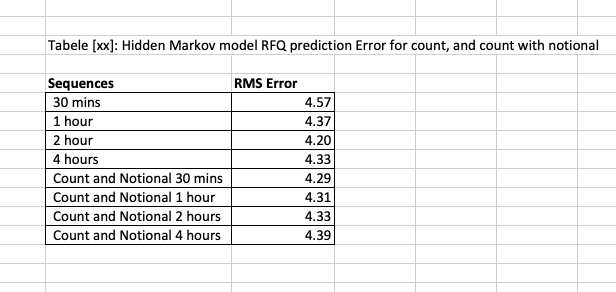
\includegraphics[width=1.0\linewidth]{./figures/Exp2_resultstable}
    \begin{tabular}{lc}
        \toprule
            Hyperparameters                  & 1D and 2D \\
        \midrule
            Distribution Inertia                   & 0.01 \\
            Maximum Iteration                     & 10.0 \\
        \bottomrule
    \end{tabular}
\end{table}



\begin{figure}[!ht]\centering
    %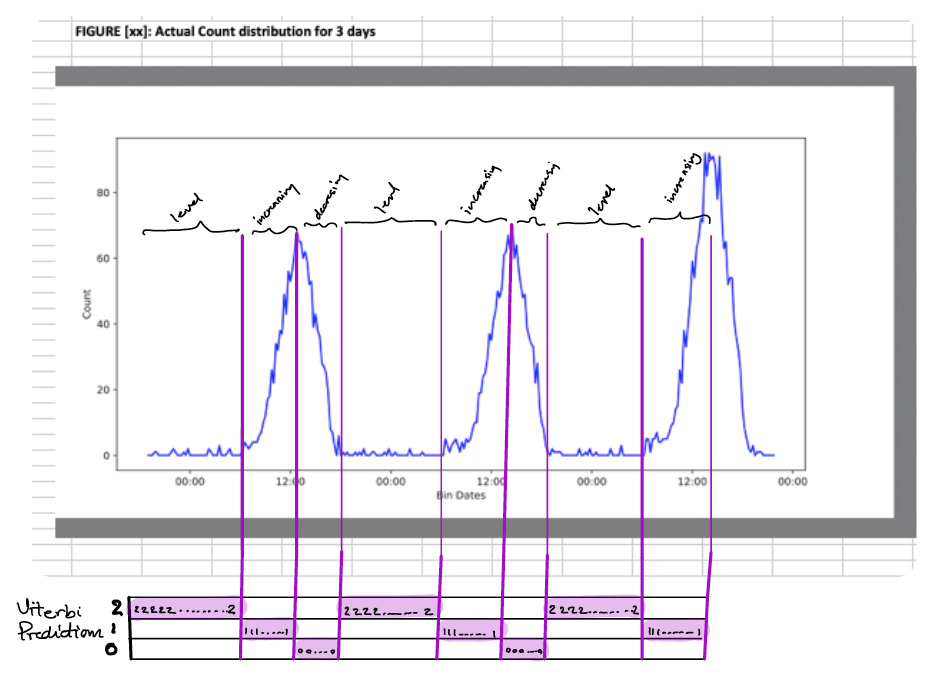
\includegraphics[width=1.0\linewidth]{./figures/Exp3_viterbi}
    \resizebox{\linewidth}{!}{\begin{tikzpicture}[x=1pt,y=1pt]
        \node[anchor=south west,inner sep=1pt] (N0) at (0,0) {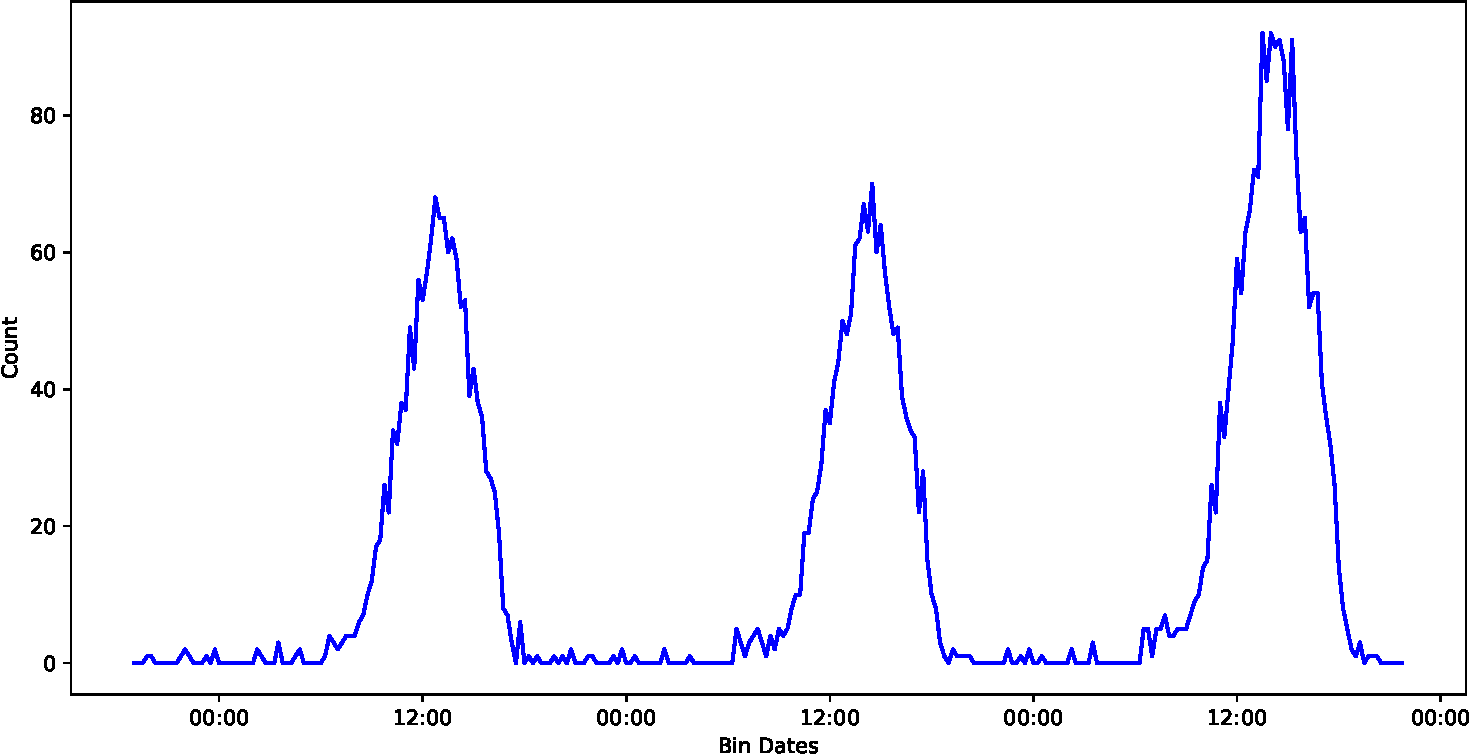
\includegraphics[width=1.0\linewidth]{./figures/Ch4fig15}};

        %\foreach \n in {0,10,20,...,500} {\draw[red,thin] (\n,0)--(\n,200) node[at start,below,scale=0.2] {\n};}

        \coordinate (Ot) at (0,220);
        \coordinate (Ob) at (0,-43);

        \coordinate (n0) at (38,0);
        \coordinate (n1) at (89,0);
        \coordinate (n2) at (120.7,0);
        \coordinate (n3) at (145.5,0);
        \coordinate (n4) at (202,0);
        \coordinate (n5) at (240.5,0);
        \coordinate (n6) at (262,0);
        \coordinate (n7) at (314,0);
        \coordinate (n8) at (350,0);
        \coordinate (n9) at (380.5,0);


        \foreach \n in {0,...,9} {\draw (n\n|-Ob)--(n\n|-Ot)
            coordinate[pos=0.00](B0\n)
            coordinate[pos=0.05](B1\n)
            coordinate[pos=0.10](B2\n)
            coordinate[pos=0.15](B3\n)
            coordinate[at end](T\n);}
        \foreach \n in {0,1,2,3} {\draw (B\n0)--(B\n9);}

        \newcommand{\bracese}[3]{\draw [decorate,decoration={brace,amplitude=5pt}] (#1.north) -- (#2.north) node [black,midway,above right,yshift=5pt,font=\footnotesize,rotate=45,inner sep=1pt] {\strut#3};}
        \newcounter{braceseci}\newcounter{bracesecii}\newcounter{braceseciii}
        \foreach \n in {0,3,6} {
            \setcounter{braceseci}{\n}\addtocounter{braceseci}{1}
            \setcounter{bracesecii}{\n}\addtocounter{bracesecii}{2}
            \setcounter{braceseciii}{\n}\addtocounter{braceseciii}{3}
            \bracese{T\n}{T\thebraceseci}{level}
            \bracese{T\thebraceseci}{T\thebracesecii}{increasing}
            \bracese{T\thebracesecii}{T\thebraceseciii}{decreasing}
            \fill[COL1,draw=black] (B2\n) rectangle (B3\thebraceseci);
            \fill[COL1,draw=black] (B1\thebraceseci) rectangle (B2\thebracesecii);
            \fill[COL1,draw=black] (B0\thebracesecii) rectangle (B1\thebraceseciii);
            \node[above,scale=0.5,inner sep=6pt] at ($(B2\n)!0.5!(B2\thebraceseci)$) {2,2,2,2,2,\dots,2};
            \node[above,scale=0.5,inner sep=6pt] at ($(B1\thebraceseci)!0.5!(B1\thebracesecii)$) {1,1,1,\dots,1};
            \node[above,scale=0.5,inner sep=6pt] at ($(B0\thebracesecii)!0.5!(B0\thebraceseciii)$) {0,0,\dots,0};
        }

        \node[left,font=\footnotesize] at ($(B20)!0.5!(B30)$) {2};
        \node[left,font=\footnotesize] at ($(B10)!0.5!(B20)$) {1};
        \node[left,font=\footnotesize] at ($(B00)!0.5!(B10)$) {0};

        \node[left,font=\footnotesize,text width=20pt,align=right] at ([xshift=-40pt]$(B10)!0.5!(B20)$) {Viterbi\\ prediction};
    \end{tikzpicture}}
    \caption{Experiment 3 -- Viterbi algorithm prediction aligned to a 3 day RFQ distribution}\label{Exp3:viterbi_pred}
\end{figure}


\begin{figure}[!ht]\centering
    %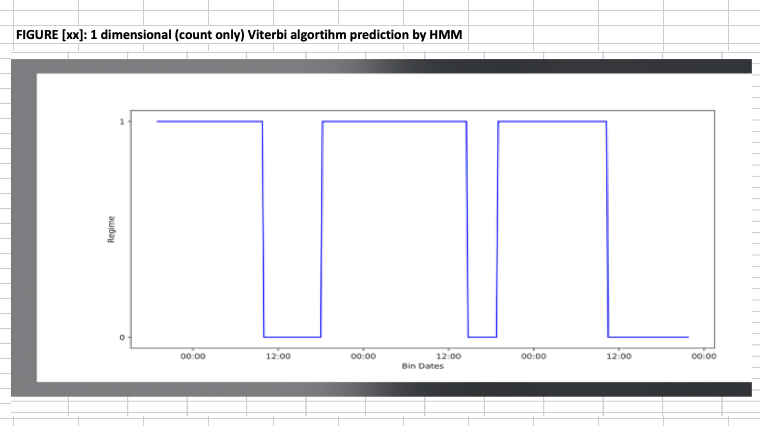
\includegraphics[width=0.8\linewidth]{./figures/Exp3_viterbi_pred_1d}
    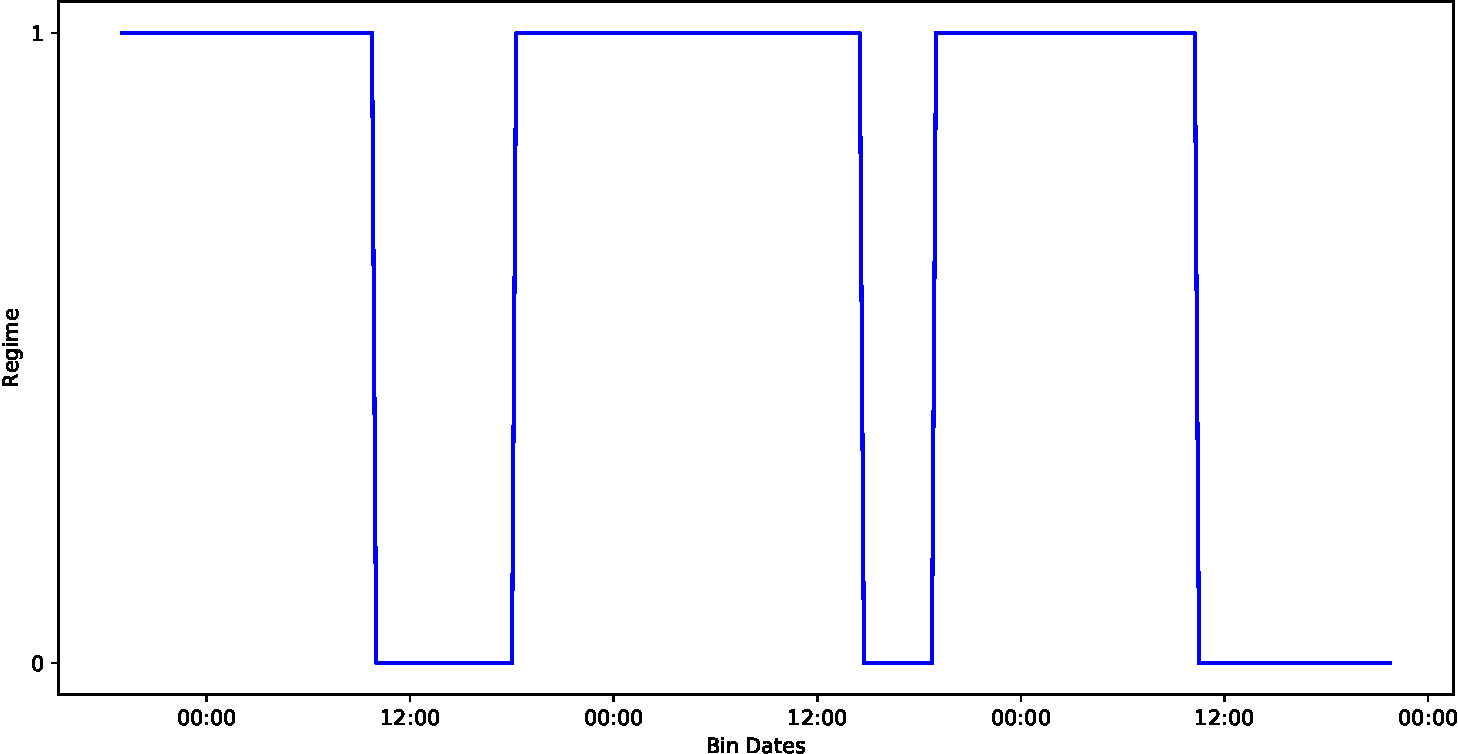
\includegraphics[width=0.8\linewidth]{./figures/Ch4fig13}
    \caption{Viterbi algorithm prediction on 1D sequence}\label{Exp3:viterbi_pred1d}
\end{figure}

\begin{figure}[!ht]\centering
    %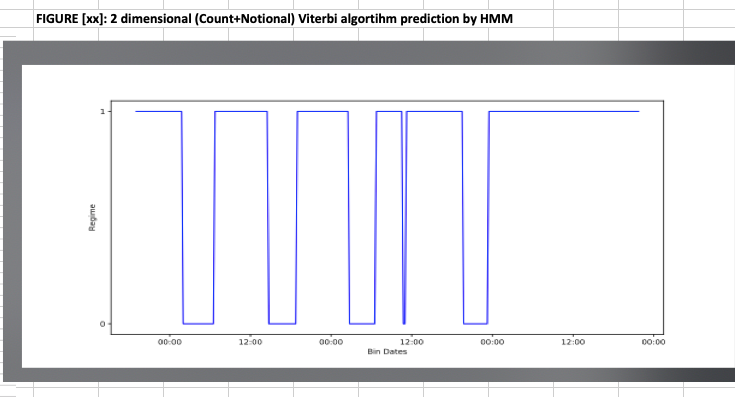
\includegraphics[width=0.8\linewidth]{./figures/Exp3_viterbi_pred_2d}
    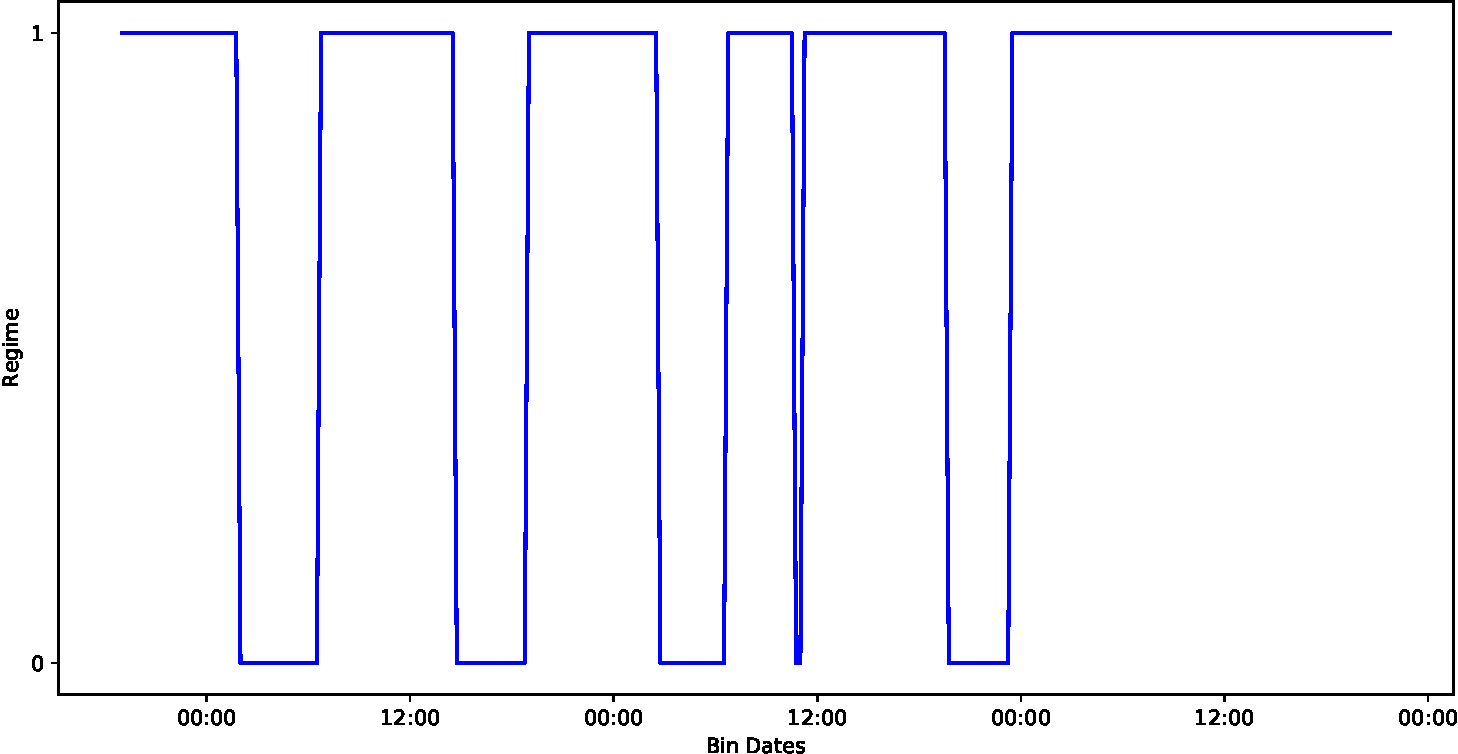
\includegraphics[width=0.8\linewidth]{./figures/Ch4fig14}
    \caption{Viterbi algorithm prediction on 2D sequence}\label{Exp3:viterbi_pred2d}
\end{figure}


\subsection{Conclusion}

Experiment 3 demonstrates that the Bayesian hidden Markov model is able to learn and infer the hidden state of the underlying visible RFQ data with good success in both 1D and 2D cases. The Viterbi predictions of the hidden states based on the `differences' align with the observed data and clearly indicate the changing regimes for both 1D and 2D sequences.